
\section{Results from the Litterature Study}

  \subsection{Password habits among web users}

    %Password reuse, frequency of webpage use (login habits), password strength, password policy

  The term ``habit'' is often a bad thing when talking about security. A habit is often hard to change and are often a predictable pattern. Password reuse is one of the known password habits among users. It is a well known problem that users tends to have an increasingly number of account that requires the users to remember yet another number of password across muliple systems and devices. The problem is not just to remember all the password needed, but also remembering which passwords that belongs to which account or device. Because of the human capacity of remembering password are causing users to choose weak passwords, as well as reuse the passwors across muliple web pages. In order to understand the users passwords habits, this section will include relevant research on users passwords habits.

  One of the first large-scale studies on web password habits was conducted in 2007 by Microsoft research \cite{habits1}. They analysed web password habits among 544960 web users over a period of 3 months. The data was collected from a Windows Live Toolbar and they observed activities like login frequency. They also collected information about the users age, the strength of the users passwords, as well as number of unique passwords and its use across different URLs. They observed that a normal user have an average of 7 distinct password and that an average of 5 of these password was re-used on different webpages. The estimate on average number of account pr user was estimated to be 25 account pr user, but this would probably be higher since it 7 years ago. 

  Password habits may be different across different subpopulation in cause of different background or culture. In 2012 Joseph Bonneau released a analysis of 70 million passwords from Yahoo! \cite{Bonneau2}. The data is analysed in terms of guessing rate by using a dictiornary attack. The collected data contained 328 subpopulations. The results showed that there was no ``good'' populations among the collected data, but there was a variation in the population. Demographically, the gender had a small effect in the guessing rate, but it showed that age tended to give effekt where password strength increases across different age groups. The analysis also showed that laguage had a significally effect on the password strength where Indonesian-speaking users were among the weakest subpopulations, and in contrast the German and Korean-speaking users provided relativley stonger passwords. 

  Passwords are not just used in our private life, but also a requirement in a critical concern from a business point of view where the use of authentication for corporate systems, mobile, and room codes plays a major role in normal day of work. In corporate systems users are often promt with the a notification frorcing them to change the password in a specified time interval. The problem with this is that user already have problems remembering their passwords as is. A reseach group conducted a questionnaire survey in a large organization \cite{habits2}. The goal was to get a understanding of password habits in a business point of view. The results showed that the users were promped with password change 7 times a year causing 68\% of the employees to re-use the same password with a minor change in order to still be able to remembering their passwords.

  \subsection{Security habits among smartphone users}

  %Intro
  Users are not only dependent on remembering passwords across multiple web pages and systems, but do also need to remember passwords for our small mobile devices. In todays society we're addicted to our mobile devices in our every day life. Mobile devices are not just a communication tool for calling and texting, but also an important tool for every day tasks like doing our work, reading mail, pay our bills and keeping up with our social life. This trend makes our mobile devices vurnerable in terms of security. To avoid unwanted access, smartphones offers different locking mechanisms. The history of locking mechanisms was often a solution solely to prevent accidental use, while current mobile phones require protection in order to secure the potentially vast amount of private data that we keep on our smartphones. Our mobile devices are in rapidly use, leading users to create and reuse shorter passwords and PINs, or no authentication at all. 

  % The time used on unlocking the phone
  In terms of security it is intersting to look at the use of mobile devices and look at the locking habits among users on mobile devices. It is known that services that are rapidly used have weaker password because of the overhad the user needs to spend on typeing their password. In 2014 a group of reasearchers published a fieild study of smartphone (un)locking behavior \cite{habits3}. Some of the problems with smartphone users tends to be their rapidly use of their phone. When the device are rabidly use, it results in a lot of time unlocking their phone between every use. In the study they found that there was a significant overhead in the time used of unlocking their phone, where the users participated in the field study used 2.9\% (9\% in the worst case) of their time unlocking their smartphone. 
  
  % The use of locking mechanisms
  Smartphones in use today do not require their users to have a locking mechanism on their smartphone. It is well known that users tends to choose to easiet way out and may result in the choice of not having any locking mechanism at all. Based on the result of the overhead in time used on unlocking their phone, a result may be to take the easiest way out by ignoring the vurlerability of not using a locking mechnismn at all. It have been discovered that over 40\% of the users only used a basic ``slide-to-unlock'' mechanism on their smartphone, as well as over 16\% didnt use any locking mechanismns at all \cite{habits3}. This highlights a major bad habit among mobile users. What happens if your mobile is stolen? 

  % Risk vs securtiy
  It is important to understand why people use or not use locking mechanisms on their smartphone. Reseach have covered that the 46.8\% of the paricipants agreed or fully agreed that unlocking their phone can be annoying, but at the same time 95.5\% of the somewhat or fully agreed that they liked the idea that their phone was protected \cite{habits3}. This highlights that the users wants to be secure, but there might be a tradeoff between the time used to unlock the smartphone vs the security risk.








    

    %How many looses their phones?
    %How much do users use their phone (measured in hours)?






  \subsection{Graphical passwords}




  \subsection{Android Unlock Pattern}

    The Android Unlock Patterns are a simplified version of the Pass-Go scheme that was proposed by Tao and Adams in 2008, and can be seen as a successor of the Draw-a-Secret (DAS) scheme. Both Pass-Go, Draw-a-Secret, and Android Unlock Patterns is categorized as recall-based authentication schemes.

    The Android password patterns are a simplified version of the Pass-Go scheme using a 3x3 grid, instead of a 9x9 as the Pass-Go scheme originally was designed. The Pass-Go scheme was inspiered from the chineese board game ``Go''.

    The settings on Android phones provides a default setting for using the Unlock pattern. 
    The rules are simple: 
        \begin{enumerate}
            \item At least four points must be chosen,
            \item You cannot vist the same node twice.
            \item Only straight lines are allowed, and
            \item One cannot jump over point not visited before
        \end{enumerate}

    \begin{figure}[H]
        \centering
        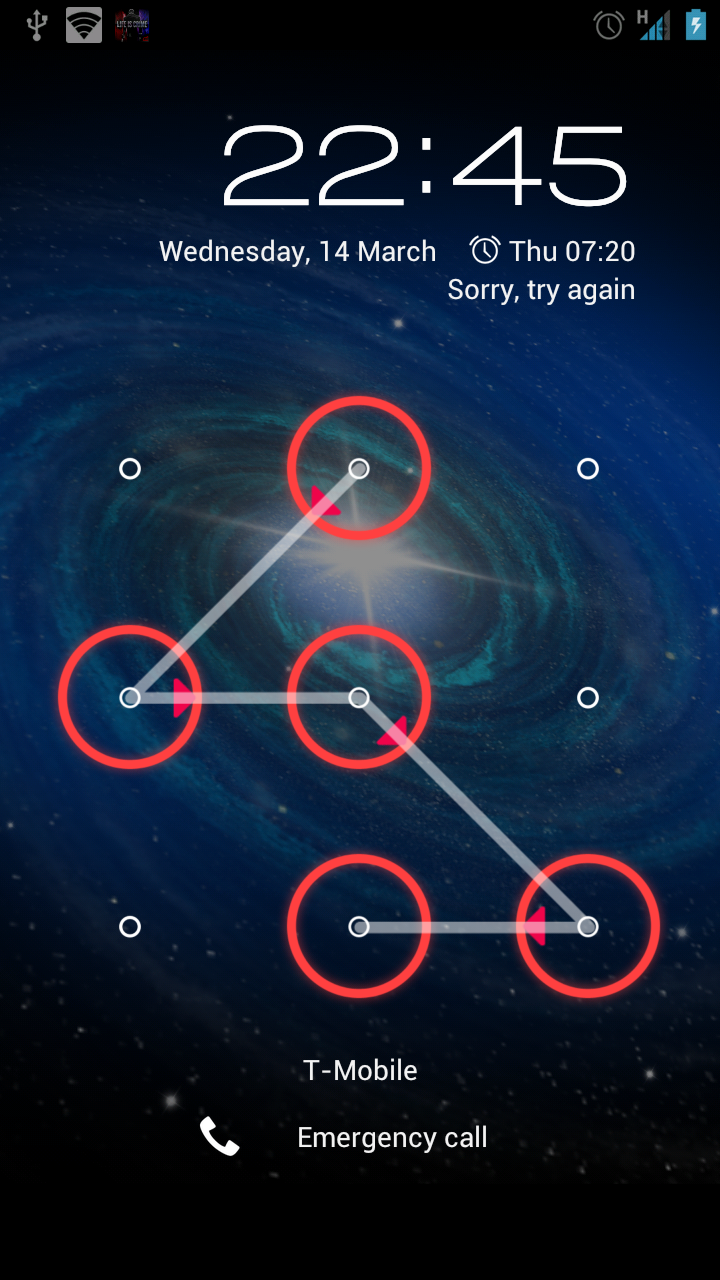
\includegraphics[scale=0.8]{pics/patternLock.png}
    \end{figure}